L'algorithme Monte Carlo Tree Search défini en \ref{alg:mcts} est un algorithme d'apprentissage par renforcement.
Il stocke en mémoire le \emph{modèle} du jeu sous forme d'arbre, et joue en fonction de ce modèle.
Dans le modèle de jeu, chaque noeud représente un état. La racine est l'état courant, et les enfants de la racines
sont les prochains états. L'algorithme stocke 2 informations essentielles par noeud: $N$ le nombre de visites du noeud, et $W$
le nombre victoires du joueur (et non de l'ennemi) en partant de ce noeud.

Il y a deux cas d'utilisations de l'algorithme : entraînement et exploitation.
Pour l'entraînement, on sélectionne une feuille de notre modèle de jeu en suivant une stratégie spécifique.
Ensuite, on regarde tous les enfants possibles depuis cet état et on en choisit un. On déroule
la partie jusqu'à arriver à un état \emph{terminal}. Le déroulement de la partie doit être le plus rapide possible.
Dans le cas de notre projet, nous avons décidé de choisir un déroulement aléatoire, même si nous aurions pû choisir une manière plus intelligente de jouer\footnote{Tel que jouer le coup qui maximise le nombre de coups possibles} qui permettrait
à l'algorithme de converger plus rapidement à une solution efficace.
Un exemple du déroulement d'une itération de l'algorithme est représenté dans la Figure \ref{fig:mcts-exemple}.
\begin{figure}[H]
	\centering
	\raisebox{-0.5\height}{
		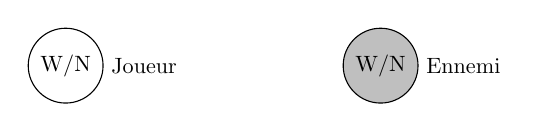
\begin{tikzpicture}[scale=0.8, every node/.style={transform shape}]
			\node (A)[draw, circle, label=right:Joueur] at (0,0) {W/N};
			\node (A)[draw, circle, fill=lightgray, label=right:Ennemi] at (5,0) {W/N};
		\end{tikzpicture}
	}
	\subfloat{
		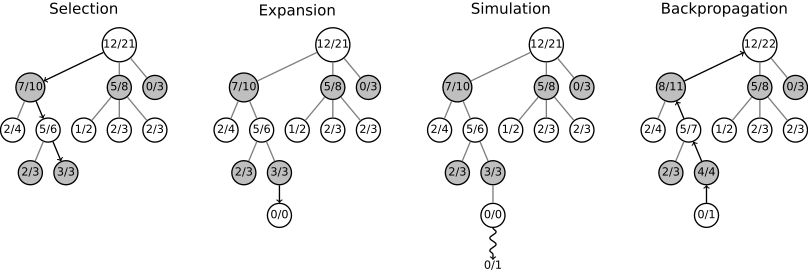
\includegraphics[width=0.9\linewidth]{MCTS_example}
	}
	\caption{Exemple d'itération de l'algorithme MCTS (\href{https://commons.wikimedia.org/wiki/File:MCTS_(French).svg}{Wikimedia})}
	\label{fig:mcts-exemple}
\end{figure}

Même si cet algorithme converge vers minmax\footnote{Bouzy, Bruno. \href{https://ewh.ieee.org/cmte/cis/mtsc/ieeecis/tutorial2007/Bruno_Bouzy_2007.pdf}{"Old-fashioned Computer Go vs Monte-Carlo Go"}. IEEE Symposium on Computational Intelligence and Games, April 1–5, 2007, Hilton Hawaiian Village, Honolulu, Hawaii.},
il nécessite un nombre d'itérations conséquent. De plus, il faut bien choisir notre heuristique grâce à laquelle on choisit notre noeud à l'étape de sélection.
Enfin, cet algorithme est en théorie meilleur que alphabeta, mais nous n'avons pas réussi à obtenir de résultats concluants.
Peut-être cela est-ce dû à une complexité de nos algorithmes trop élevée. Ou dû au fait que durant l'expansion, nous
simulons tous les enfants. 

Une amélioration possible serait d'évaluer les enfants du noeud sélectionné de façon parallèle.
En effet, les zones mémoires sont séparés, nous pouvons donc plutôt facilement paralléliser le problème.
Même après moultes profilages et optimisations, l'algorithme du MCTS n'a malheureuseent pas été concluant, malgré
toutes les promesses à son propos\dots

\begin{algorithm}
	\Entree{p: plateau, A: arbre de jeu}
	\Deb{
		$to\_expand \gets selection(A)$\;
		$expansion = expand(to\_expand)$\;
		$result = simulate(expandison)$\;
		$backpropagate(result, A, expansion)$\;
	}
	\caption{Algorithme Monte Carlo Tree Search}
	\label{alg:mcts}
\end{algorithm}